\chapter{Конструкторский раздел}
\label{cha:design}

В данном разделе будут рассмотрены схемы алгоритмов и структура реализации.

\section{Схемы алгоритмов сортировки}
На рисунке ~\ref{fig:edge_flag} приведена схема алгоритма заливки полигона.
На рисунке ~\ref{fig:dda} приведена схема алгоритма отрисовки отрезка.
На рисунке ~\ref{fig:thread} приведена схема параллельного рендеринга.

\begin{figure}
    \centering
    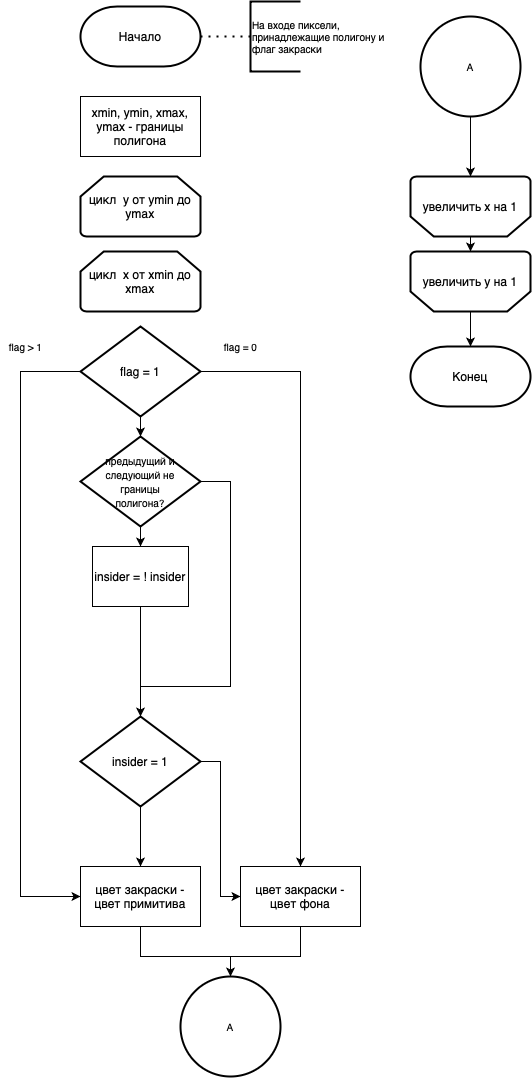
\includegraphics[height=0.75\textheight]{sem-v-aa-master/lab1/tex/inc/schemes/lab3.drawio.png}
    \caption{Схема алгоритма заливки полигона}
    \label{fig:edge_flag}
\end{figure}

\begin{figure}
    \centering
    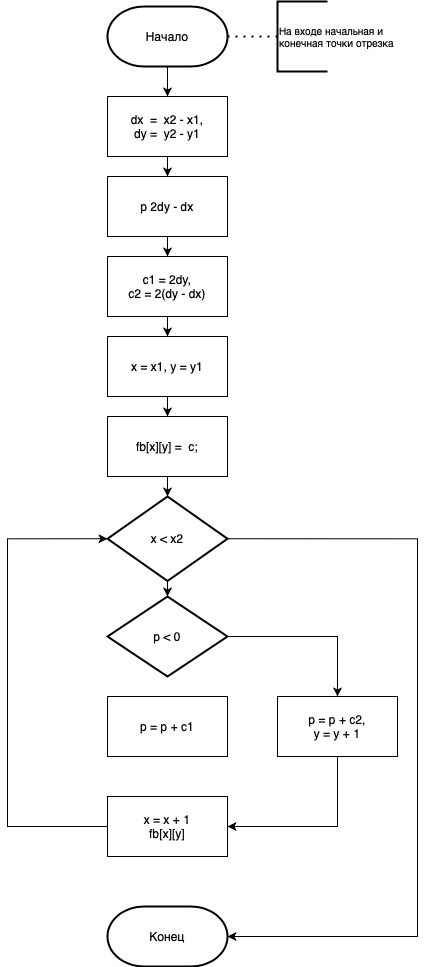
\includegraphics[height=0.75\textheight]{sem-v-aa-master/lab1/tex/inc/schemes/lab3-dda.png}
    \caption{Схема алгоритма DDA отрисовки отрезка}
    \label{fig:dda}
\end{figure}

\begin{figure}
    \centering
    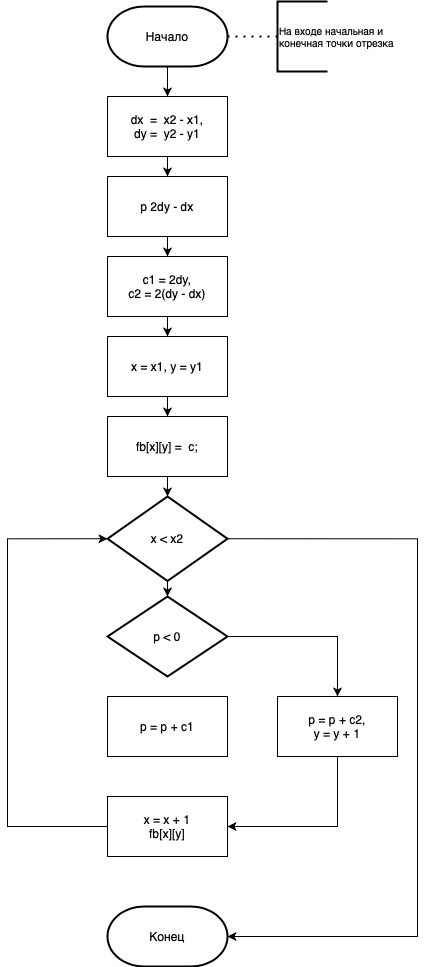
\includegraphics[height=0.75\textheight]{sem-v-aa-master/lab1/tex/inc/schemes/lab3-dda.png}
    \caption{Схема алгоритма DDA отрисовки отрезка}
    \label{fig:dda}
\end{figure}

\begin{figure}
    \centering
    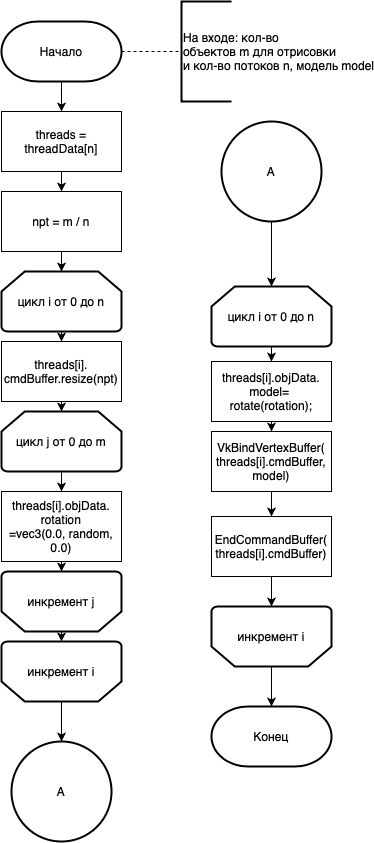
\includegraphics[height=0.75\textheight]{sem-v-aa-master/lab1/tex/inc/schemes/lab4.drawio.png}
    \caption{Схема параллельного рендеринга}
    \label{fig:thread}
\end{figure}
    
\section{Вывод}

На основе теоретического материала из аналитического раздела были построены схемы реализаций исследуемых алгоритмов.

%%% Local Variables:
%%% mode: latex
%%% TeX-master: "rpz"
%%% End:
